\chapter{Antennas} % (fold)
\label{cha:antennas}

\section{Antennas Parameters} % (fold)
\label{sec:antennas_parameters}

\subsection{Directive Gain} % (fold)
\label{sub:directive_gain}

The power radiated by an antenna depends on the direction. The \textit{directive gain} toward a given direction is expressed as:

\begin{equation}
	D ( \theta, \phi) = \frac {Radiation \ \ Intensity} {Isotropic \ \ Intensity } = 	    \frac{ U(\theta , \phi)} {P_{rad}/ 4\pi}
\end{equation}

% subsection directive_gain (end)

\subsection{Directivity function and $D_M$ definition} % (fold)
\label{sub:_d_m_}

There is a direction $(\theta_{MAX},\phi_{MAX})$ where D is maximum. The directivity function is the function D normalized to $D_M$:

\begin{equation}
	f(\theta,\phi)=\frac{ \textit{D}(\theta,\phi)}{D_M} \ \ \ \Longrightarrow S_R(R,\theta,\phi)= \frac{P_{rad}}{4\pi R^2} D_M f(\theta,\phi)
\end{equation}

$D_M$ represents the ratio between the radiated power density in the direction where it is maximum divided by the power density obtained with an isotropic radiator:

\begin{equation}
	D_M=\frac{4 \pi }{ \int_0^{2\pi}\int_0^{2\pi} f(\theta,\phi)sin(\phi) d\theta d\phi}
\end{equation}

% subsection _d_m_ (end)

\subsection{Radiated Power Density} % (fold)
\label{sub:radiated_power_density}

It is usefull to evaluate the radiated power density as it can be used for an analysis of propagation of power towards the threedimensional space.

\begin{equation}
	S_R=\frac{dP_{rad}}{ds}=\frac{1}{2}Re(E\times H^*)=\frac{1}{R^2}\textit{U}(\theta,\phi)
\end{equation}

\subsubsection*{Isotropic Radiation}

In case of isotropic radiation the radiation intensity $\textit{U}(\theta,\phi)= \frac{P_{rad}}{4\pi}$ 

\subsubsection*{Non Isotropic Radiation}

In non isotropic cases we get that the radiotion intensity is:

\begin{equation}
\textit{U}(\theta,\phi)= \frac{P_{rad}}{4\pi} \textit{D}(\theta, \phi)
\end{equation}


The radiated power intensity results:
\begin{equation}
S_R(R,\theta,\phi)= \frac{P_{rad}}{4\pi R^2} \textit{D}(\theta, \phi)
\end{equation}

From the formula of the power density at distance R we can derive the net radiated power:

\begin{equation}
	P_{rad}= \iint_{\Sigma} S_R(R, \theta, \phi)\, d\Sigma = \frac{P_{rad}D_{MAX}}{4 \pi R^2}\iint_{\Sigma} f(\theta, \phi) \, d\Sigma
\end{equation}


\begin{figure}[h]
	\centering
	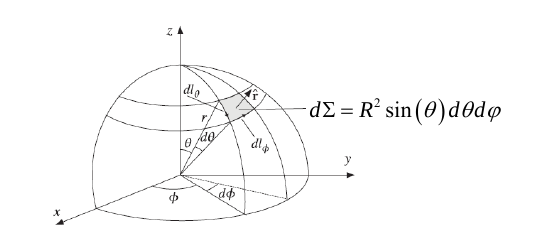
\includegraphics[scale=0.6]{Immagini/sph}	
	\label{fig:sph}
\end{figure}

\begin{equation}
	P_{rad} = \frac {P_{rad}D_{MAX}}{4 \pi}\int_0^{ \pi}\int_0^{2 \pi} \sin(\theta) f(\theta, \phi) d\theta d\phi
\end{equation}

from which:

\begin{equation}
	\frac{1}{D_{MAX}}=\frac{\eta}{G}= \frac{1}{4 \pi} \int_0^{\pi}\int_0^{2 \pi} \sin(\theta) f(\theta, \phi) d\theta d\phi
\end{equation}

and :

\begin{equation}
	G =\frac { 4\pi \eta}{\int_0^{ \pi}\int_0^{2 \pi} \sin(\theta) f(\theta, \phi) d\theta d\phi}
\end{equation}
% subsection radiated_power_density (end)

\subsection{Fields Intensity} % (fold)
\label{sub:fields_intensity}

The radiated Power can be also related to the intensity of the electromagnetic fields:

\begin{equation}
	S_R=\frac{1}{2}\frac{\sqrt{\epsilon_r}}{Z_0}|E|^2= \frac{1}{2}\frac{Z_0}{\sqrt{\epsilon_r}}|H|^2
\end{equation}

The power density from a transmitting antenna (PT , G)
at distance R along the direction of maximum radiation
is given by: 

\begin{equation}	
S_R= \frac{P_TG}{4 \pi R^2}
\end{equation}


Then:

\begin{equation}
	|E| = \frac{1}{R} \sqrt{\frac{Z_0 P_{ERP}}{2\pi \sqrt{\epsilon_r}}} \ \ \ [V/m]
\end{equation}


\begin{equation}
	|H| = \frac{1}{R} \sqrt{\frac{\sqrt{\epsilon_r} P_{ERP}}{2\pi Z_0}} \ \ \ [A/m]
\end{equation}
% subsection fields_intensity (end)


\subsection{Efficienty of Antennas} % (fold)
\label{sub:efficienty_of_antennas}

The impedance “seen” by the transmitter is determined by 2 contributes: $Z_R$ \footnote{radiation impedance} and $R_p$ \footnote{loss resistance}. The power dissipated by $Z_R$ constitutes the radiated power\footnote{Typically $R_p \ll |Z_R|$}.

Assuming the reader aware of maximum power transfer theorem, neglecting the losses resistances because as stated before negligible in respect of the radiation impedence, we will assume impedence matching.

To understand how much of the electrical power is actually translated in radiated power the antenna efficiency can be defined as:

\begin{equation}
  	\eta = \frac{P_{rad}}{P_T}= \frac{Re\{ Z_R \}}{Re\{ Z_R \}+R_p}
  \end{equation}  

% subsection efficienty_of_antennas (end)

\subsection{Effective Radiated Power} % (fold)
\label{sub:effective_radiated_power}

The effective radiated power if simply defined as:

\begin{equation}
	P_{ERP} = P_TG 
\end{equation}


\subsection{Gain of Antennas} % (fold)
\label{sub:gain_of_antenna}

Defined as:

\begin{equation}
	G = \eta D_M
\end{equation}

the gain is one of the fundamental paraments that describes an antenna.

% subsection gain_of_antenna (end)
% subsection effective_radiated_power (end)

\subsection{Received Power} % (fold)
\label{sub:received_power}


\begin{figure}[h]
	\centering
	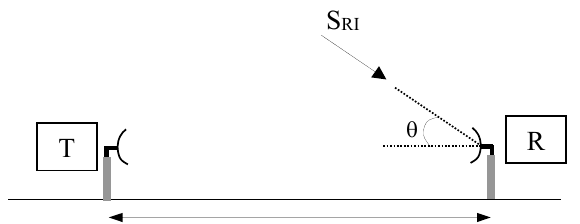
\includegraphics[scale=0.3]{Immagini/SR}
	
	\caption{Simplified scheme of a Radio Link with an additiona power density from an non optimal direction}
	\label{fig:SR}
\end{figure}

Given the power density ($S_R$)\footnote{magnitude of the Poynting vector} and the direction of arrival ($ \theta $) of an incident radiation the received power can be calculated as:

\begin{equation}
	P_r=A_{\textit{e}} S_R f(\theta)
\end{equation}

where:

\begin{itemize}
	\item $A_{\textit{e}}$ is the \textbf{effective Area} of the anttenna
	\item $f(\theta)$ is the directivity function

\end{itemize}


% subsection received_power (end)


\subsection{Effective Area} % (fold)
\label{sub:effective_area}



\begin{equation}
	\frac{G}{A_e}=\frac{4 \pi }{\lambda^2}
\end{equation}

% subsection effective_area (end)


\subsection{Equivalent length} % (fold)
\label{sub:equivalent_length}

The equivalent length can be related to the effective area using the following formula:



% subsection equivalent_length (end)



% section antennas_parameters (end)


\section{Radio Link} % (fold)
\label{sec:radio_link}


\subsection{Link Budget} % (fold)
\label{sub:link_budget}

\begin{figure}[h]
	\centering
	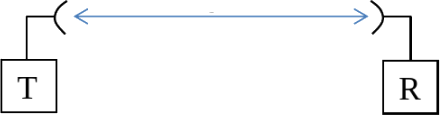
\includegraphics[scale=0.6]{Immagini/link}
	
	\caption{Simplified scheme of a Radio Link}
	\label{fig:link}
\end{figure}

Supposing to have a Radio Link as in Figure~\ref{fig:link} between 2 Antennas at a certain relative distance R the link budget may be evaluated by means of the \textbf{Friis equation} which at the end leds to a simple analitical expression for the receiving power\footnote{which is the logaritmic form of the Friis equation}:

\begin{equation}	
P_{r|_{dB}} = P_{t|_{dB}} - 10 \log{frac{\lambda}{4\pi R}} + G_{t|_{dB}} + G_{r|_{dB}} 
\end{equation}

in which:

\begin{itemize}
	\item $P_{r|_{dB}}$ is the effective power received by the antenna.
	\item $P_{t|_{dB}}$ is the overall transmitted power of the TX side.
	\item $G_{r|_{dB}}$ is the gain of the receiving antenna.
	\item $G_{t|_{dB}}$ is the gain of the transmitting antenna.
\end{itemize}

while the term $20\log{ \frac{\lambda}{4 \pi R} }$ stands for the free space losses.
Note from a practical point of view there as at least a couple of DoF in the design flow to obtain a certain receiving power.

We may also report the linear form of the \textbf{Friis equation}:

\begin{equation}
P_r = P_t  \left( \frac { \lambda } {4 \pi L}^2 \right) G_T G_R
\end{equation}


% subsection link_budget (end)


\subsection{Attenuators' Noise} % (fold)
\label{sub:noise_of_attenuators}

In any RF receiver we are going to have at least some losses between the antenna and the LNA. Sometimes also in other sections of the receiver path attenuation couldn't be avoided.
We may evaluate the additional noise introduced my an attenuator $A_{f1}$ for example the one in Figure~\ref{fig:Teq} as:

\begin{equation}
	T_{f1} = T_0 (10^{ \frac {A_{f1}} {10} }-1)
\end{equation}

% subsection noise_of_attenuators (end)



\subsection{Equivalent Temperature} % (fold)
\label{sub:equivalent_temperature}

\begin{figure} [h!]
	\centering
	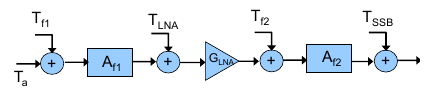
\includegraphics[scale=1]{Immagini/Teq}
	
	\caption{General structure of a noisy receiving chain}
	\label{fig:Teq}
\end{figure}


Supposing to have a receiving chain as in Figure\footnote{note that here $A_x$ stands for an attenuation $= \frac{1}{Gain}$ and G stands for a Gain}~\ref{fig:Teq} we may want to rappresent the system with noiseless components and an input referred noise considering all contribution.
This could be very usefull beacuse using this model the Signal-to-Noise Ratio evalutation turns out to be extremly simple, while we can just compare the receiving power with the overall noise directly at the input port.

To get an $T_{equivalent}$ we have to refer at the input any additional noise by dividing it by the Gain from to input to the point where the noise is injected.

At the end for the example in figure we get:

\begin{equation}
	T_{sys}=T_{eq}= T_a + T_{f1} + T_{LNA} A_{f1}+ T_{f2} \frac { A_{f1} } {G_{LNA}} + T_{SSB} \frac { A_{f1} A_{f2} } {G_{LNA}}
\end{equation}

where:
\begin{itemize}
	\item $T_{f1}$ is the noise introduced by the first attenuator
	\item $T_{LNA}$ is the noise introduced by the LNA
	\item $T_{f2}$ is the noise introduced by the second attenuator
	\item $T_{SSB}$ is the noise introduced by the mizer
\end{itemize}
With the same concept we may find the \textit{Output Referred Noise} $T_out$ by simply applyng the relative transfer function at each noise to the ouput:

\begin{equation}
	T_out = T_a\frac {G_{LNA}} {A_{f1} A_{f2} } + T_{f1}\frac { G_{LNA}} {A_{f1}A_{f2}} + T_{LNA}\frac{G_{LNA}}{A_{f2}}+ T_{f2}\frac{1}{A_{f2}} + T_{SSB} 
\end{equation}

and to get $T_{eq}$ we may divide $T_{out}$ by the noiseless gain $\frac{G_{LNA}}{A_{f1}A_{f2}}$

\begin{equation}
	T_{eq}=\frac{T_out}{\frac{G_{LNA}}{A_{f1}A_{f2}}}
\end{equation}

after some algebra it's clear that the two different approaches are absolutely equivalent.

% subsection equivalent_temperature (end)


\subsection{Noise Figure} % (fold)
\label{sub:noise_figure}

The Noise Figure is very usefull as it gives an immediate evaluation of the overall degration that a system gives to the SNR.

Noise Figure is usually  calculate diving the overall noise of the system by the noise given by the source; this operation is usually done at the output but can be done in every point of the system.

% subsection noise_figure (end)

\subsection{Noise figue and equivalent temperature relationship} % (fold)
\label{sub:noise_figue_and_equivalent_temperature_relationship}


\begin{equation}
	T_{eq}= T_0(10^{\frac{NF_{eq}}{10}}-1)
\end{equation}

where $T_0$ it's usually the room temperature considered $290^{\circ}C$.
% subsection noise_figue_and_equivalent_temperature_relationship (end)


\subsection{Datarate Limitation} % (fold)
\label{sub:datarate_limitation}


Given the modulation and demodulation scheme\footnote{Given the mod/demod scheme the energy transmitter per bit is fixed}, the bandwidth (B) and the minimum SNR required the maximum possible datarate (R) is limited by noise.

Known the equivalent noise temperature ($T_{eq}=T_{sys}$) e can write:

\begin{equation}	
SNR = \frac{P_r}{KT_{sys}B}=\left(\frac{E_b}{N_0}\right)\left(\frac{R}{B}\right)
\end{equation}


% subsection datarate_limitation (end)

% section radio_link (end)

% chapter antennas (end)





\chapter{Receivers} % (fold)
\label{cha:receivers}


\section{Image} % (fold)
\label{sec:image}

The problem of the image rises during the domodulation process when the RF signal is downconverted to an Intermediate Frequncy (IF) because of the mixer by means of the LO downconverts to IF both the RF signal and the Image which any signal at the same opposite distance\footnote{Note that this deistance is by definition IF} from the LO with respect to RF signal.

\subsection*{Example} % (fold)
\label{sub:example}

Let's report an example for clarification\footnote{$1^{st}$ February 2017 exercise 1 question a)}:
\begin{itemize}
	\item $f_{RF}= 12 Ghz$ 
	\item $f_{IF}= 140 Mhz$ 
\end{itemize}

we know that the local oscillator frequency (fLO) is above the signal band.

Find the frequncy of the image is quite simple:


\begin{equation}
	f_{IF}=|f_{RF}-f_{LO}|
\end{equation}

from this we are able to find $f_{LO}$ and then:

\begin{equation}
		f_{IM}=f_{LO}-f_{IF}= f_{RF}-2f_{IF}
\end{equation}

\section{Cascaded Noise Figure} % (fold)
\label{sec:cascaded_noise_figure}

The evalutation of the Noise figure of cascaded stage could be performed with this formula:

\begin{equation}
	NF_{eq}= NF_1 + \frac{NF_2-1}{G_1} + \frac{NF_3-1}{G_1G_2} 
\end{equation}

% section cascaded_noise_figure (end)



% subsection example (end)

% section image (end)

% chapter receivers (end)